\documentclass[letterpaper,journal]{IEEEtran}
\usepackage{amsmath,amsfonts}
\usepackage{algorithmic}
\usepackage{array}
\usepackage[caption=false,font=footnotesize,labelfont=sf,textfont=sf]{subfig}
\usepackage{textcomp}
\usepackage{stfloats}
\usepackage{url}
\usepackage{graphicx}
\usepackage{cite}
\usepackage{booktabs}
\usepackage{multirow}

\begin{document}

\title{Simplified PD+Feedforward Line-Following Robot with Radar Avoidance and LoRa Telemetry}

\author{
    \IEEEauthorblockN{Yujia Lin\textsuperscript{1}, Ziyi Zhu\textsuperscript{2}, Mengzhuo Xu\textsuperscript{3}, Zijin Mu\textsuperscript{4}, and Yuxuan Liang\textsuperscript{5}} \\

    \IEEEauthorblockA{\textsuperscript{1}GUID 2960092, \textsuperscript{2}GUID 2960283, \textsuperscript{3}GUID 2960183, \textsuperscript{4}GUID 2960297, \textsuperscript{5}GUID 2960351\\
    Team 15 PTSD\\
    }
}

\markboth{Team 15: TDPS Final Report, June~2026}%
{Y.~Lin \textit{et al.}: TDPS Line-Following Robot}

\maketitle

\begin{abstract}
This paper presents an autonomous line-following robot that integrates radar obstacle avoidance and LoRa checkpoint telemetry on a single STM32F407VET6 microcontroller without an RTOS. Root-cause failure analysis of a legacy 62-parameter PID system identifies seven mutually competing mechanisms that render systematic tuning infeasible, motivating a simplified 6-parameter PD plus curvature feedforward (PD+kff) architecture. We optimize parameters through two-round systematic sweeping (63 groups) on an offline simulator that compiles the identical C control code against a physics harness, achieving a 30--40$\times$ speedup over on-car testing. The optimal configuration achieves a simulator regression score of 97.65/100 with 100\% line detection and zero off-line time; the feedforward term reduces steering correction standard deviation by 19\% versus pure PD control. A bounded-trigger communication strategy confines TOF measurement and LoRa transmission to stable straight-course windows, preventing wireless reporting from interfering with high-risk turning or recovery states. On-car validation confirms stable tracking on straights, curves, and U-turns. We analyze the dual role of the 22\,cm sensor preview distance --- simultaneously a damping advantage and a junction-handling challenge --- as a design trade-off that extends beyond this platform.
\end{abstract}

\begin{IEEEkeywords}
Line following, PD control, curvature feedforward, radar avoidance, LoRa telemetry, embedded systems.
\end{IEEEkeywords}

\section{Introduction}

\IEEEPARstart{T}{he} University of Glasgow Team Design Project (TDPS) requires each team to design a robot that completes three tasks --- line-following, radar obstacle avoidance, and LoRa checkpoint telemetry --- on a single microcontroller without an operating system. Meeting this requirement on an STM32F407VET6 (Cortex-M4, 168\,MHz)~\cite{cortex_m4_trm} demands not only individual subsystem competence but also their coexistence within a deterministic 10\,ms control loop, making integration the primary challenge~\cite{siegwart2011autonomous, astrom1995pid}.

\subsection{Problem Statement and Scope}

Three tightly coupled constraints govern the design. First, the 22\,cm sensor preview --- the distance between the sensor array and the drive axle --- simultaneously provides natural derivative damping and creates a geometric mismatch at junctions and U-turns that no gain tuning can resolve. Second, the HLK-LD2410S 24\,GHz radar provides only forward distance information without lateral discrimination, so obstacle avoidance must rely on timed open-loop maneuvers with heuristic direction selection. Third, LoRa checkpoint reporting shares the same bare-metal execution context as line following; the EWM22A module requires AUX busy-state polling before UART transmission, and the paired TOF query also introduces blocking serial latency. The core engineering tension is between control-loop timing, sensor geometry, and communication latency --- three constraints that must be satisfied simultaneously.

The scope is explicitly bounded: this project addresses a single differential-drive robot with a fixed sensor configuration. Multi-robot coordination, visual SLAM, and adaptive road-surface detection are outside scope.

\subsection{Literature Survey}

Line-following on resource-constrained microcontrollers has been explored through several control paradigms. Classical PID control~\cite{astrom1995pid} remains prevalent due to its minimal computational requirements~\cite{braunl2006embedded}, yet established tuning methods such as SIMC~\cite{skogestad2003simple} assume sensor--actuator co-location --- an assumption violated when the sensor is physically separated from the drive wheels. Alternative paradigms (fuzzy logic, model predictive control) relax parameter sensitivity or achieve higher tracking performance, but sacrifice analytical transparency or demand floating-point computation budgets unavailable on a Cortex-M4 running bare-metal firmware.

Integrating sensing and communication on a shared microcontroller introduces additional constraints. Single-chip 24\,GHz mmWave radar modules~\cite{ld2410s_datasheet} provide compact range sensing but are inherently forward-only, precluding closed-loop lateral correction during obstacle circumvention. LoRa communication~\cite{lorawan_spec, ewm22a_datasheet} offers long-range, low-power data links at the expense of low data rates and AT-command blocking latencies that conflict with hard real-time control. Existing literature addresses these components individually but does not resolve their simultaneous integration under a 10\,ms control loop on a single microcontroller without an RTOS. This work simplifies and co-optimizes the control, sensing, and communication subsystems within these coupled constraints.

\subsection{Report Structure}

Section~II presents the system-level design approach and architectural rationale. Section~III details each subsystem's design and the motivation behind key decisions. Section~IV reports quantitative experimental results. Section~V provides cross-cutting analysis of design trade-offs, concludes with key findings, and identifies future directions.

\section{Overall System Design Approach}

\subsection{System Architecture Overview}

The system adopts a layered Perception--Control--Actuation--Communication architecture orchestrated by a single-threaded main loop with peripheral interrupts. We employ a tick-based non-blocking design rather than cooperative scheduling or a preemptive RTOS~\cite{labrosse2002rtos}. The task set comprises three bounded periodic sources --- a 10\,ms line-sensor sampling tick, a radar UART parser at approximately 20\,Hz, and discrete LoRa checkpoint events --- each with measured worst-case execution time well below the main-loop period. A cooperative scheduler would add explicit yield points without improving temporal isolation for this small task set, and an RTOS would introduce scheduling jitter and stack overhead; a bare-metal super-loop is the simplest deterministic solution. Fig.~\ref{fig:architecture} illustrates the four-layer architecture.

\begin{figure}[!t]
    \centering
    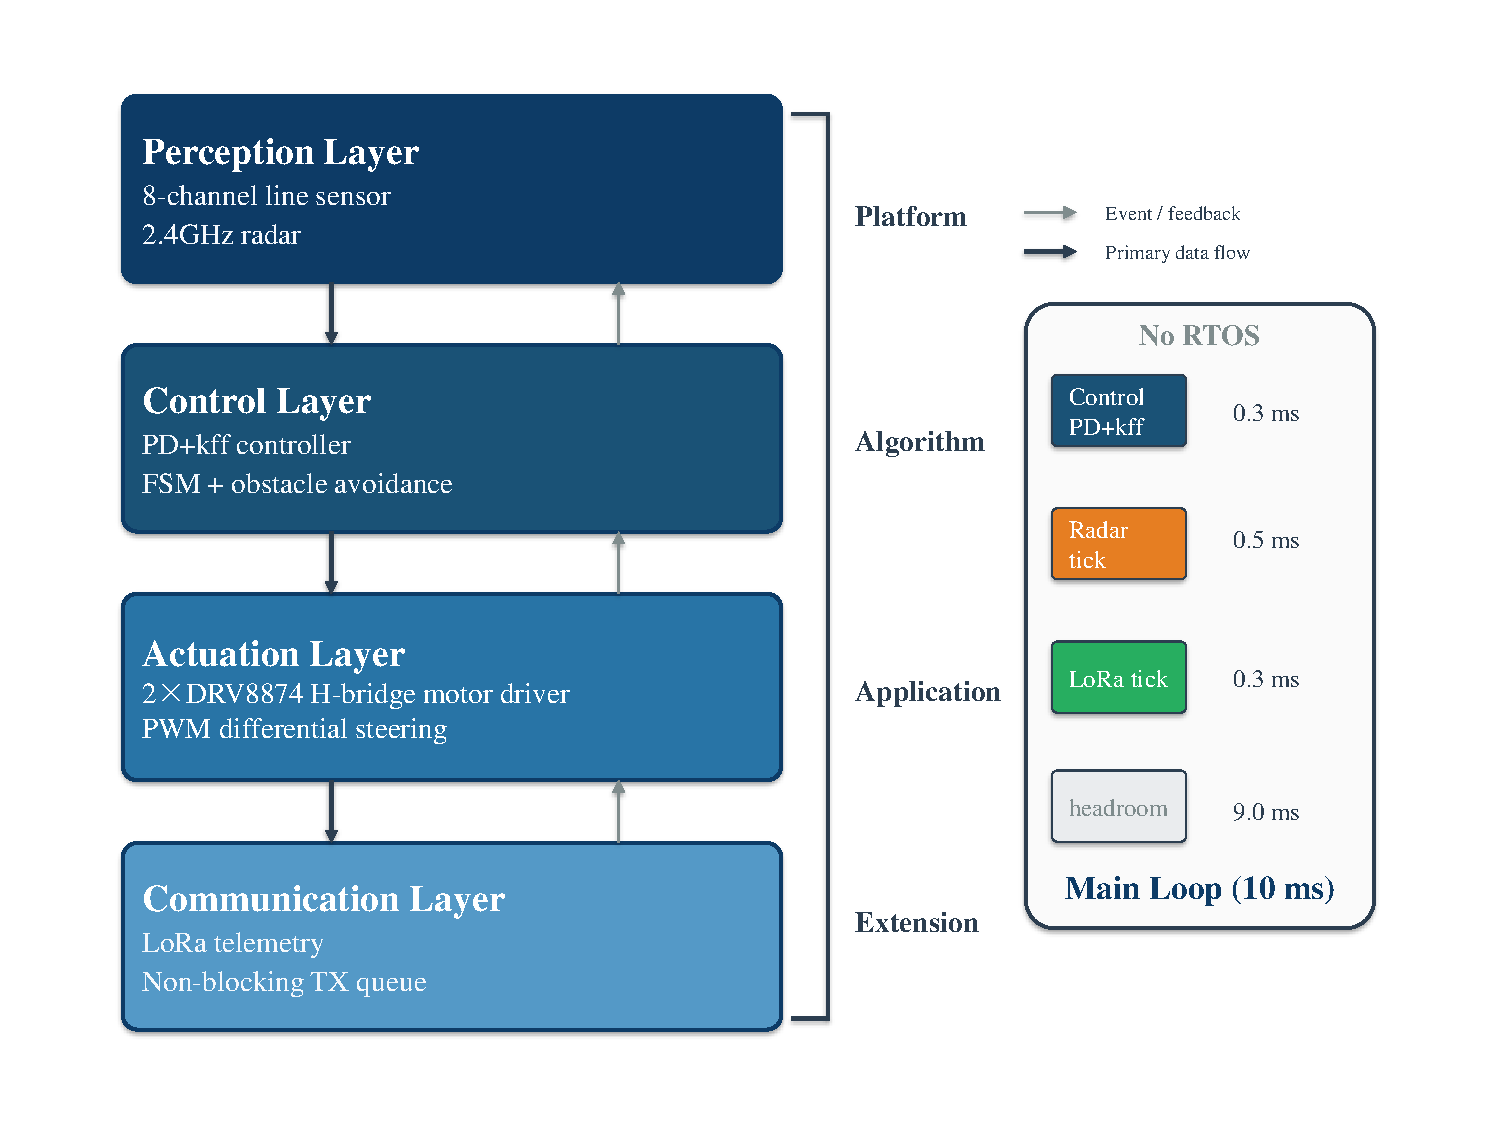
\includegraphics[width=\linewidth]{figures/fig1_architecture.pdf}
    \caption{Four-layer system architecture. We organize the firmware into Perception, Control, Actuation, and Communication layers, orchestrated by a single-threaded 10\,ms main loop with peripheral interrupts. The Communication layer performs gated LoRa checkpoint reporting, restricting transmission to stable straight-course windows.}
    \label{fig:architecture}
\end{figure}

\begin{figure}[!t]
    \centering
    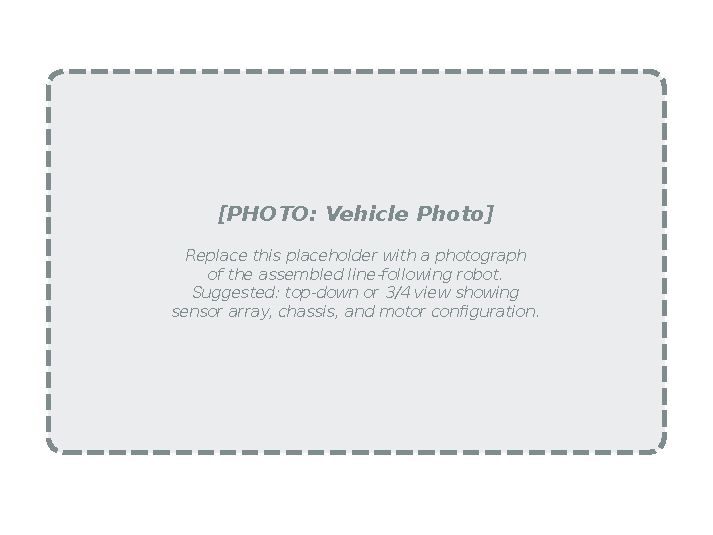
\includegraphics[width=\linewidth]{figures/fig2_vehicle_photo.pdf}
    \caption{Assembled differential-drive platform. The 8-channel sensor array mounts 22\,cm ahead of the drive axle, providing preview damping at the cost of geometric mismatch at junctions. The HLK-LD2410S radar, EWM22A LoRa module, and STM32F407VET6 controller share a custom four-layer power regulation PCB.}
    \label{fig:vehicle}
\end{figure}

The four software layers --- Platform, Algorithm, Application, and Extension --- enforce interface boundaries: Platform isolates STM32 HAL dependencies, Algorithm contains portable sensor processing and control logic, Application owns the state machine, and Extension contains radar and LoRa peripheral services invoked only through guarded application states. This layering prevents wireless activity from preempting turning or recovery. Fig.~\ref{fig:vehicle} shows the assembled physical platform.

\subsection{Hardware Platform and Constraints}

The robot uses a differential-drive chassis with a 16\,cm wheel track. An 8-channel Yahboom grayscale sensor array communicates via UART at 9600\,baud and mounts 22\,cm ahead of the drive axle center --- a geometry that directly governs the relationship between sensor measurements and vehicle position. HLK-LD2410S 24\,GHz radar and EWM22A-900BWL22S LoRa modules connect via separate UART interfaces. The STM32F407VET6 (Cortex-M4, 168\,MHz, 512\,KB Flash, 192\,KB SRAM) serves as the central controller~\cite{stm32f407_ref}. Table~\ref{tab:hw-specs} summarizes the key hardware components.

\begin{table*}[!t]
    \caption{Hardware Component Specifications}
    \label{tab:hw-specs}
    \centering
    \footnotesize
    \begin{tabular}{@{}p{0.09\textwidth}p{0.16\textwidth}p{0.22\textwidth}@{}}
        \toprule
        \textbf{Subsystem} & \textbf{Component} & \textbf{Specifications} \\
        \midrule
        MCU & STM32F407VET6 & Cortex-M4, 168\,MHz, 512\,KB Flash \\
        Line Sensor & Yahboom 8-LP & 8-ch, UART 9600\,baud \\
        Radar & HLK-LD2410S & 24\,GHz, 0.75--6\,m, 115200\,baud \\
        LoRa & EWM22A-900BWL22S & 868/915\,MHz, UART5 fixed-point mode \\
        Motor Driver & 2$\times$DRV8874PWPR & 3.6\,A peak \\
        Power & LM2596S $+$ AMS1117 & 5\,V/3\,A $+$ 3.3\,V LDO \\
        \bottomrule
    \end{tabular}
\end{table*}

The power subsystem uses a two-stage regulation chain --- an LM2596S buck converter (5\,V/3\,A) followed by an AMS1117-3.3 LDO --- with an LM74700 reverse-polarity protection controller and NTMFS5C628NLT1G MOSFET at the battery input. All regulation, protection, MCU, motor drivers, and interface components share a single custom four-layer PCB detailed in Section~\ref{subsec:pcb}.

\subsection{PCB Design and Integration}
\label{subsec:pcb}

We designed and fabricated a custom four-layer PCB integrating all core electronics --- MCU, power regulation, motor drivers, sensor interfaces, and radio headers --- on a single 100$\times$100\,mm board. The board consolidates the STM32F407VET6 with 8\,MHz oscillator and SWD header; an LM2596S buck (5\,V/3\,A) and AMS1117-3.3 LDO two-stage power chain; LM74700 reverse-polarity protection controlling an NTMFS5C628NLT1G MOSFET; two DRV8874PWPR motor drivers with bulk decoupling; and UART headers for the Yahboom sensor array, HLK-LD2410S radar, and EWM22A LoRa module. A dedicated inner-layer ground plane keeps the bill of materials to 32 components. Fig.~\ref{fig:pcb_layout} shows the PCB layout and Fig.~\ref{fig:schematic} the full schematic.

\begin{figure}[!t]
    \centering
    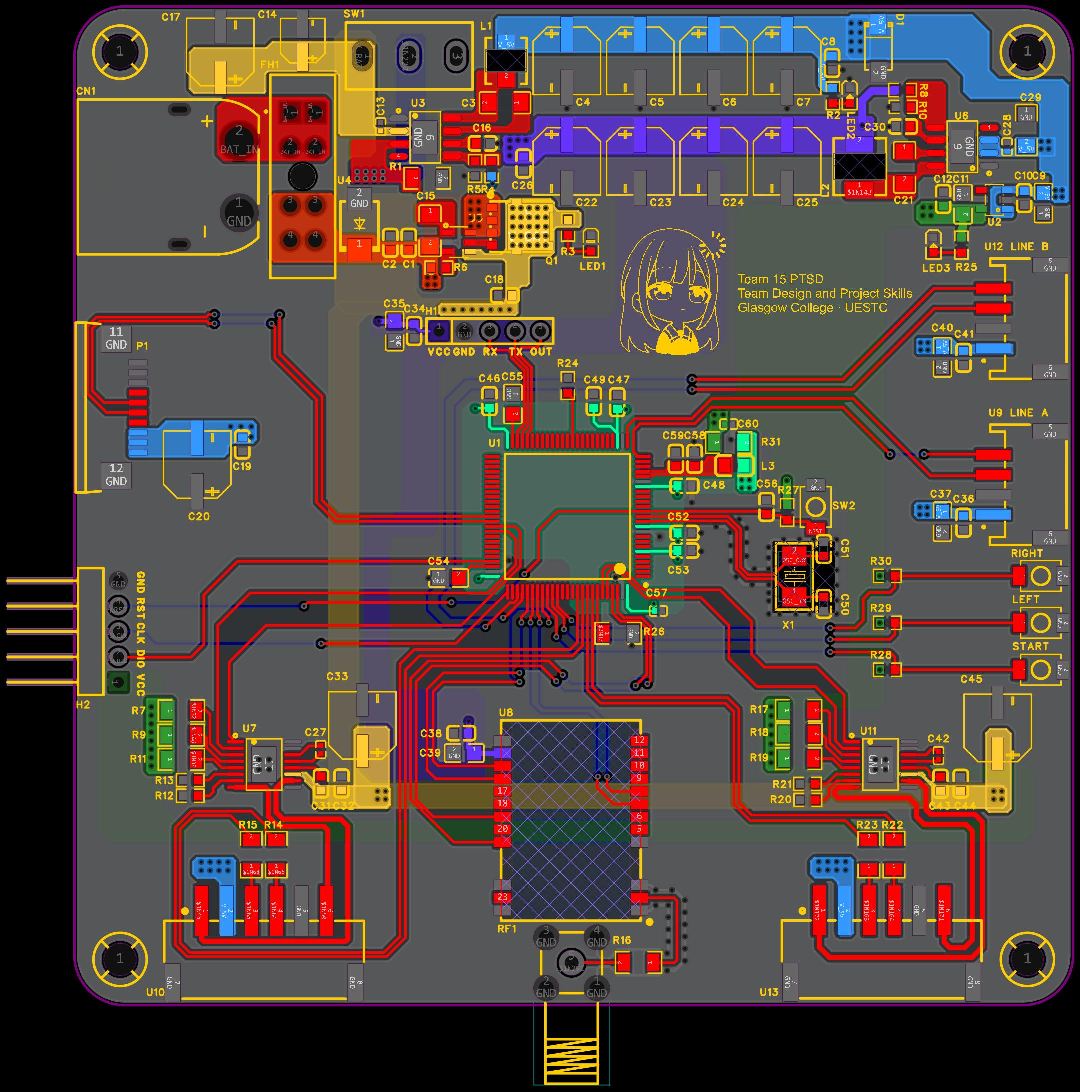
\includegraphics[width=\linewidth]{figures/fig3_pcb.pdf}
    \caption{Four-layer PCB layout. The 100$\times$100\,mm board integrates STM32F407VET6 (center-left), LM2596S buck (top), DRV8874 motor drivers (bottom), and peripheral headers along the edges. Inner layers provide dedicated power and ground planes; power traces for the motor-current path use 1.2\,mm width.}
    \label{fig:pcb_layout}
\end{figure}

\begin{figure*}[!t]
    \centering
    \subfloat[Sheet 1 --- battery input protection, LM2596S buck, AMS1117-3.3 LDO, DRV8874 motor drivers, sensor/radio UART headers.]{%
        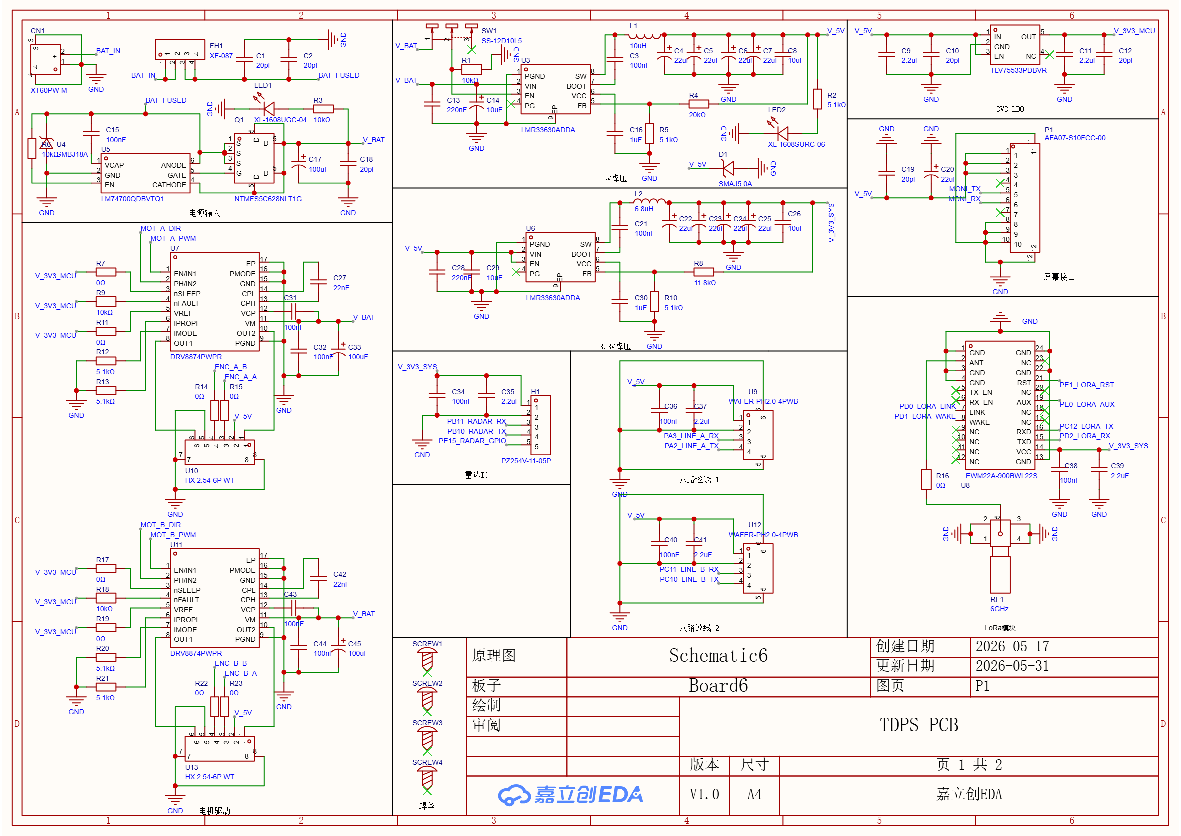
\includegraphics[width=0.48\textwidth]{figures/fig3a_sch1.pdf}%
        \label{fig:schematic_sheet1}%
    }
    \hfill
    \subfloat[Sheet 2 --- STM32F407VET6 MCU with decoupling capacitors, 8\,MHz external oscillator, and SWD debug header.]{%
        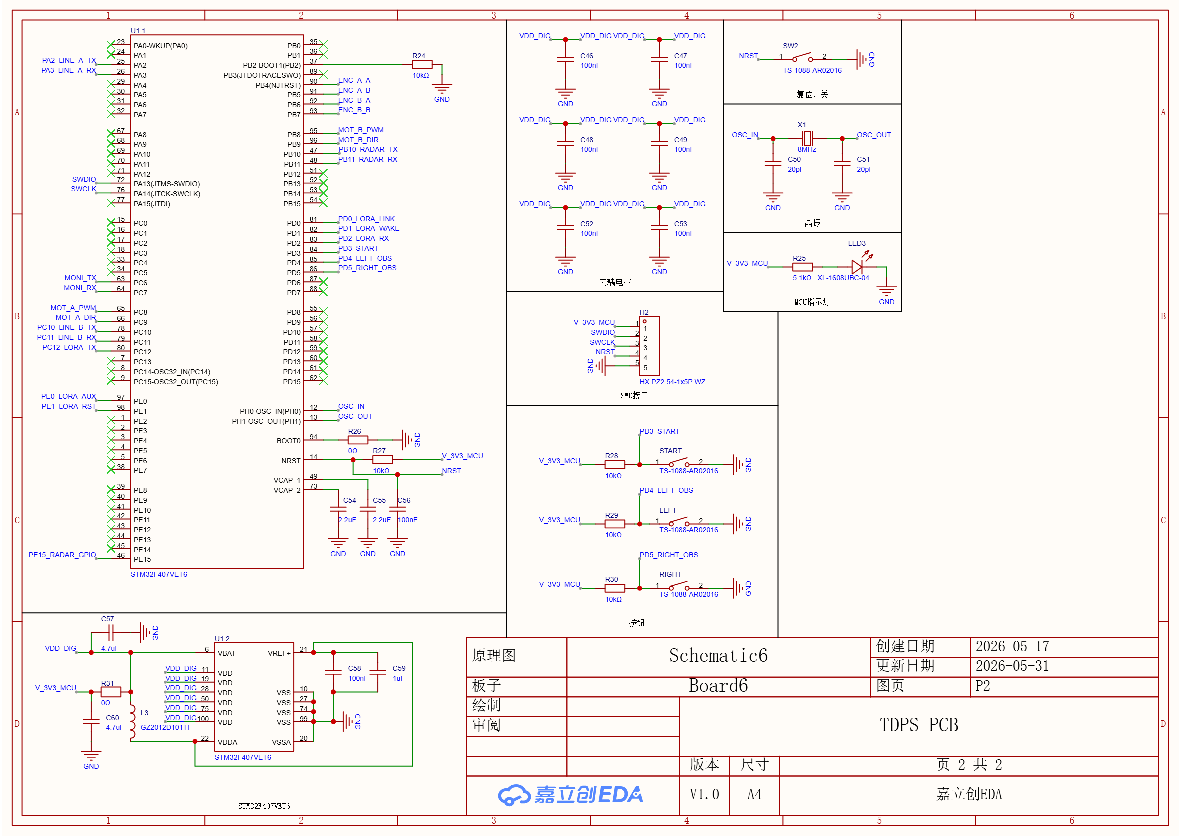
\includegraphics[width=0.48\textwidth]{figures/fig3b_sch2.pdf}%
        \label{fig:schematic_sheet2}%
    }
    \caption{PCB schematic (two sheets). (a) Power regulation, motor drivers, and peripheral interfaces --- battery protection $\rightarrow$ LM2596S $\rightarrow$ AMS1117-3.3, DRV8874$\times$2, Yahboom/HLK-LD2410S/EWM22A headers. (b) STM32F407VET6 MCU with decoupling, 8\,MHz HSE oscillator, and SWD programming interface.}
    \label{fig:schematic}
\end{figure*}

The design went through two fabrication revisions. V1 validated the core power-regulation topology and motor-driver placement but exhibited ground-bounce noise on sensor UART lines under full motor load, traced to a shared ground return path. V2 corrected this with a single-point star-ground connection under the AMS1117, reducing sensor noise below the detection threshold. V2 added reverse-polarity protection (LM74700~+~MOSFET) after a battery hot-swap damaged a V1 board.

\subsection{Geometric Constraints}

Two geometric constraints govern the control design. The 22\,cm sensor preview means that detected line features lead the drive wheels by a duration proportional to $22/v_{\text{phys}}$, where $v_{\text{phys}}$ is the physical ground speed in cm/s; this provides natural preview damping via the derivative term but requires explicit lead compensation at sharp junctions. The 16\,cm wheel track constrains the minimum differential speed required for a given turning radius.

\subsection{Project Planning and Workflow}

Development followed six milestones (M1--M6) across 24 weeks, with simulator-based validation running in parallel with on-car testing from week 5 onward. Fig.~\ref{fig:timeline} presents the full Gantt timeline.

M1 (weeks~1--4) established the hardware baseline: chassis assembly, UART peripheral verification, GPIO motor control, and PWM speed regulation. M2 (weeks~4--6) implemented the basic PID-based line follower with a discrete state machine for start/stop sequencing. M3 (weeks~10--14) added line-loss detection and recovery logic with configurable grace periods. M4 (weeks~14--17) integrated the EWM22A LoRa module with AT-command queuing, AUX-pin polling, and checkpoint-aware transmission scheduling. M5 (weeks~17--21) incorporated radar obstacle detection with a timed avoidance maneuver, which exposed the fragility of the 62-parameter controller under the combined timing pressure of three concurrent subsystems. This motivated the architecture refactoring (week~16 marker in Fig.~\ref{fig:timeline}) that reduced the control parameter set from 62 to 6. M6 (weeks~21--24) performed full three-task integration testing with joint line-following, radar avoidance, and LoRa telemetry running concurrently.

Two features of this workflow merit emphasis. First, the off-car simulator ran continuously from week~5 as a regression safety net --- every control-parameter change was validated against 16 baseline scenarios before on-car deployment, catching regressions within 30\,s rather than after a 15--20\,min physical test cycle. Second, the 62$\rightarrow$6 architecture refactoring at week~16 was enabled by simulator throughput: the coarse-to-fine 63-group sweep, which would have required days of on-car testing, completed in under one hour on the simulator, providing the quantitative evidence needed to justify eliminating 56 parameters.

\begin{figure}[!t]
    \centering
    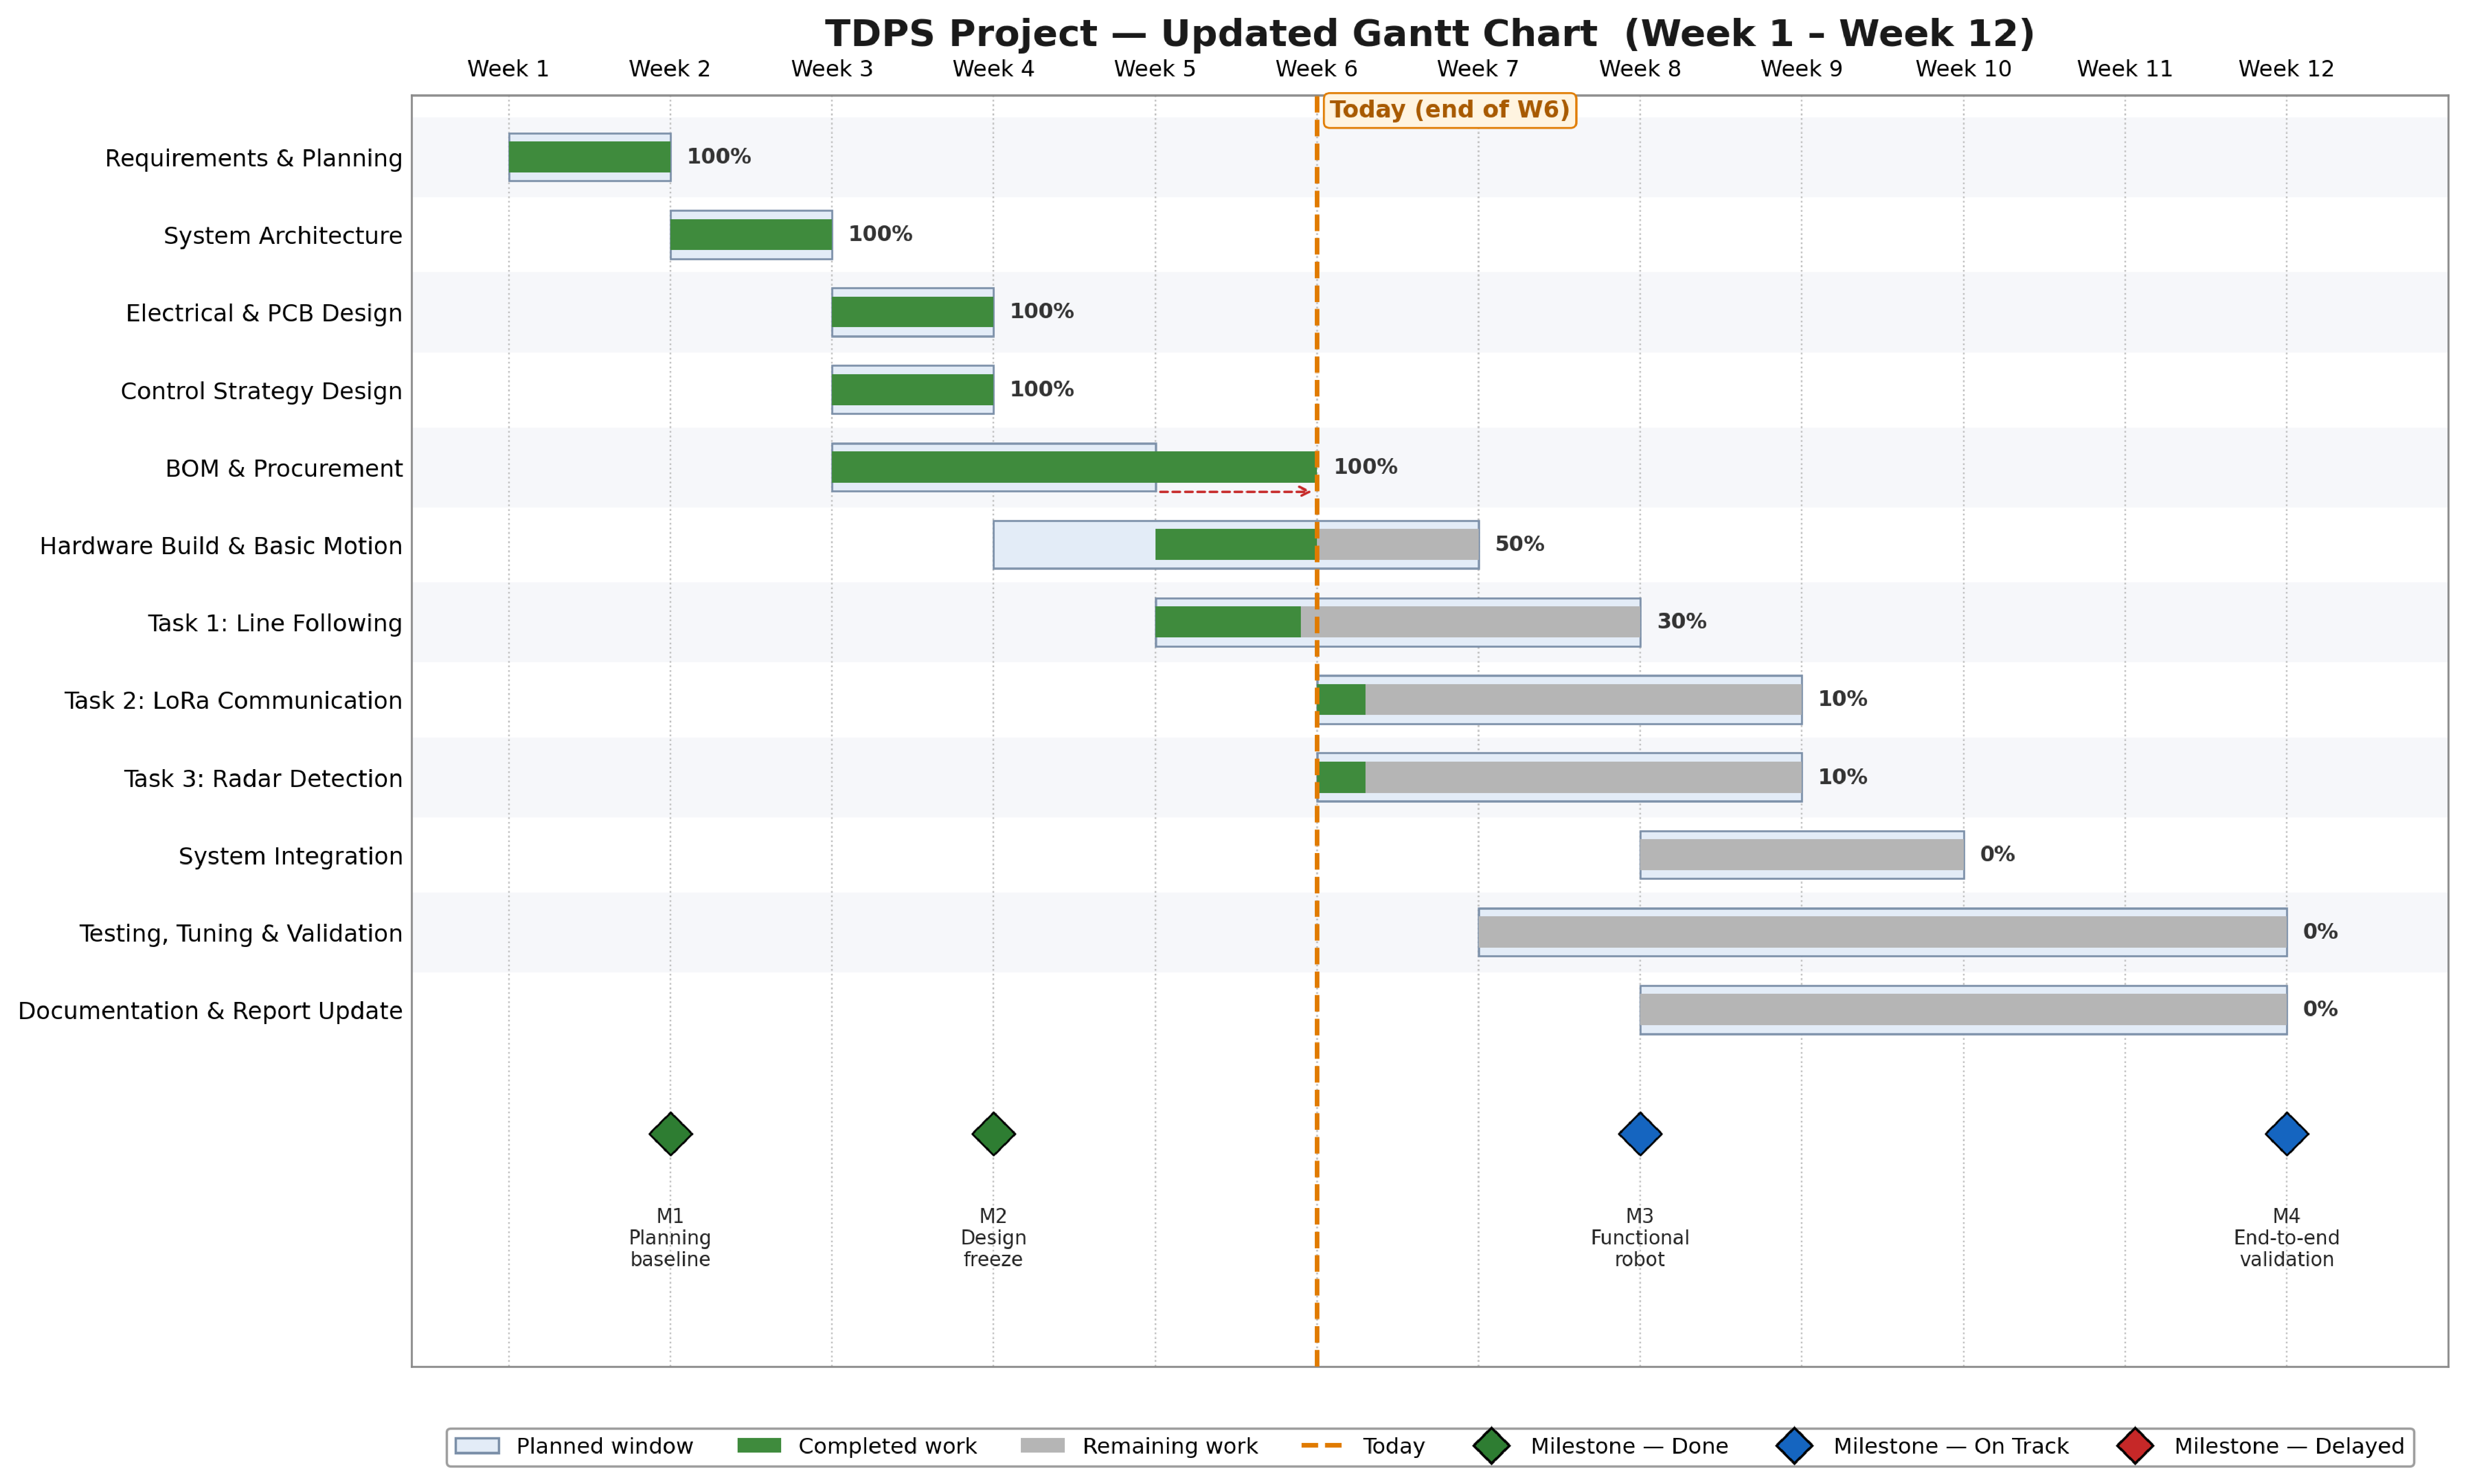
\includegraphics[width=\linewidth]{figures/fig5_timeline.pdf}
    \caption{Project timeline (24-week Gantt chart). Six milestones span chassis bring-up through full-system integration. The architecture-refactoring marker (week~16, dashed red) denotes the 62$\rightarrow$6 parameter reduction triggered by M5 radar-integration pressure. The simulator regression safety net (orange bar) ran in parallel with on-car testing (gray bar) from week~5.}
    \label{fig:timeline}
\end{figure}

\subsection{Offline Simulation and Regression Strategy}
\label{subsec:sim}

The offline simulation harness compiles the identical C control code (via GCC for PC, not cross-compiled for STM32) against a modeled environment. Each test scenario uses a CSV configuration specifying track geometry (circle, figure-8, patio, or full-competition map), initial vehicle pose, and fault-injection parameters. Vehicle dynamics use a first-order inertial model with the physical 16\,cm wheel track for trajectory integration. The virtual 8-channel sensor computes per-channel readings from ground-truth position and injects configurable Gaussian noise, multiplicative gain error, additive bias, and dropout events.

Rather than a single pass/fail threshold, the harness enforces progressive quality gates. The quick gate ($\sim$30\,s) runs all 16 baseline scenarios, requiring overall score $\geq$82, detection rate $\geq$94\%, and max off-line time $\leq$0.35\,s. The stability gate ($\sim$5\,min) repeats scenarios with 10 random seeds, requiring worst-case score $\geq$80. The full-course gate ($\sim$2\,min) tests the complete competition map at competition speed with sequential checkpoint triggering and zero-collision requirements.

The regression score $S \in [0, 100]$ uses a penalty-based formula: $S = 100 - P_{\text{det}} - P_{\text{err}} - P_{\text{lost}} - P_{\text{sat}}$, where $P_{\text{det}} = (1 - r_{\text{det}}) \times 60$, $P_{\text{err}} = \min(\bar{e}/0.08,\; 1) \times 20$, $P_{\text{lost}} = \min(t_{\text{lost}}/1.2,\; 1) \times 15$, and $P_{\text{sat}} = \min(r_{\text{sat}}/0.6,\; 1) \times 5$, with weights reflecting task priority: detection dominates (line loss is unrecoverable), cross-track error penalizes tracking quality, and line loss/saturation penalize robustness.

Measured against the prior on-car cycle of 15--20 minutes per single-track evaluation, the simulator evaluates each configuration across all 16 scenarios in approximately 30 seconds --- a 30--40$\times$ throughput improvement enabling the complete 63-group parameter sweep within a single session.

To verify correctness at multiple levels of abstraction, we employ a three-tier testing strategy (Table~\ref{tab:test-coverage}): PC-stub compilation against GCC verifies that core algorithms are free of STM32-specific dependencies and can be exercised without hardware; the Python simulator compiles the identical C control code and executes it against modeled vehicle dynamics with configurable noise and fault injection; and board-level debugging via ST-Link SWD confirms peripheral-level correctness on the actual STM32F407VET6.

\begin{table*}[!t]
    \caption{Multi-Level Test Coverage Matrix}
    \label{tab:test-coverage}
    \centering
    \footnotesize
    \begin{tabular}{@{}p{0.14\textwidth}p{0.06\textwidth}p{0.05\textwidth}p{0.05\textwidth}p{0.18\textwidth}@{}}
        \toprule
        \textbf{Test Level} & \textbf{LF} & \textbf{LoRa} & \textbf{Rdr} & \textbf{Setup} \\
        \midrule
        PC Stub (gcc) & \checkmark & \checkmark & --- & GCC compile; core algorithm verification \\
        \addlinespace
        Simulator (Python) & \checkmark & \checkmark & \checkmark & Python harness; CSV scenario, noise injection \\
        \addlinespace
        Board-Level (MCU) & \checkmark & --- & \checkmark & ST-Link SWD; peripheral verification \\
        \bottomrule
    \end{tabular}
\end{table*}

\section{Experimental Design --- Subsystem Design and Solution(s)}

\subsection{Line-Following Subsystem}

\subsubsection{Sensor Processing Pipeline}

The 8-channel Yahboom sensor communicates via UART, outputting 8 bytes per frame of grayscale intensity. The processing pipeline applies three stages: (1) \emph{ambient-light invariance} --- per-channel normalization against min/max calibration values from an initial swing-sweep; (2) \emph{noise rejection} --- a first-order IIR low-pass filter ($\alpha=0.35$); and (3) \emph{sub-sensor resolution} --- a weighted centroid $e = \sum w_i \cdot \text{norm}_i / \sum \text{norm}_i$ with linearly distributed weights, producing a continuous position signal whose effective resolution exceeds the 8 discrete sensor elements. Line presence uses a multi-condition AND of signal sum, peak value, and contrast thresholds, preventing false detection from floor artifacts. Fig.~\ref{fig:sensor} summarizes the complete pipeline.

\begin{figure}[!t]
    \centering
    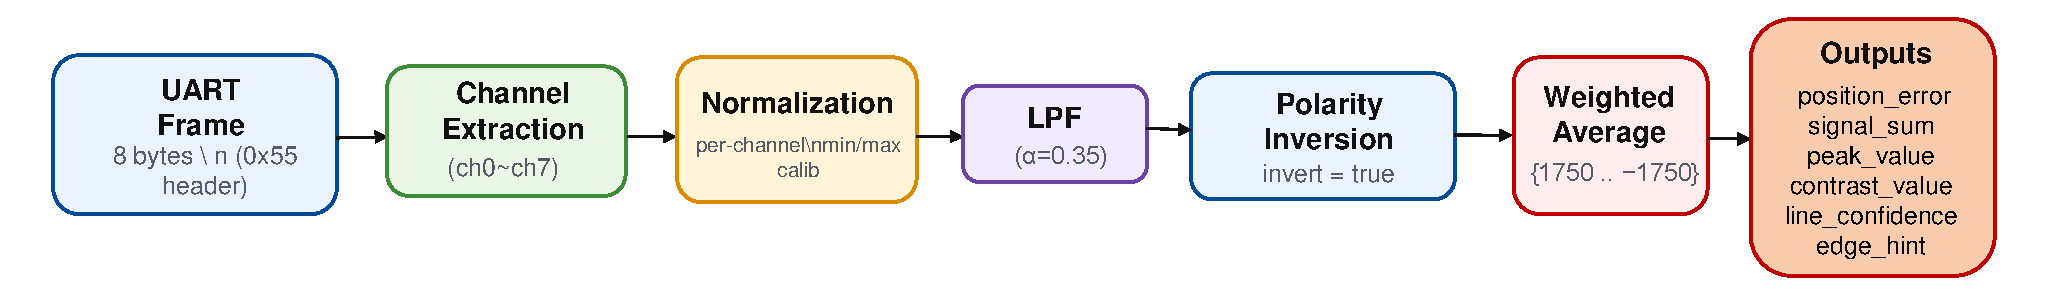
\includegraphics[width=\linewidth]{figures/fig4_sensor_pipeline.pdf}
    \caption{Sensor processing pipeline. We convert the 8-byte UART frame into a continuous position error $e$ through per-channel normalization, a first-order IIR low-pass filter ($\alpha=0.35$), and a weighted centroid computation whose effective resolution exceeds the 8 discrete sensor elements. Auxiliary quality signals (line presence, peak, contrast) support downstream loss recovery and noise rejection.}
    \label{fig:sensor}
\end{figure}

\subsubsection{Simplified PD + Curvature Feedforward Controller}
\label{subsec:controller}

The controller uses a simplified 6-parameter architecture that computes steering correction as:
%
\begin{equation}
    \text{correction} = k_p \cdot e + k_d \cdot \dot{e} + k_{\text{ff}} \cdot \dot{e} \cdot v
    \label{eq:correction}
\end{equation}
%
where $e$ is the weighted position error (dimensionless, range $[-1750, 1750]$, where 1750 is the maximum absolute centroid value), $\dot{e}$ is its discrete-time derivative, and $v$ is the smoothed vehicle speed in PWM duty-cycle counts (range 0--500, corresponding to 0--100\% duty cycle). The vehicle speed follows a continuous function of position error:
%
\begin{equation}
    v = v_{\text{base}} - (v_{\text{base}} - v_{\text{min}}) \cdot \frac{|e|}{1750}
    \label{eq:speed}
\end{equation}
%
with IIR smoothing ($\alpha=0.4$). All speed and correction values are in PWM counts (range 0--500, corresponding to a 0--100\% duty cycle with ARR\,=\,499). Differential commands $v_L = v + \text{correction}$, $v_R = v - \text{correction}$ are individually clamped by $C_{\text{max}}=300$. Fig.~\ref{fig:control} presents the control block diagram.

\begin{figure}[!t]
    \centering
    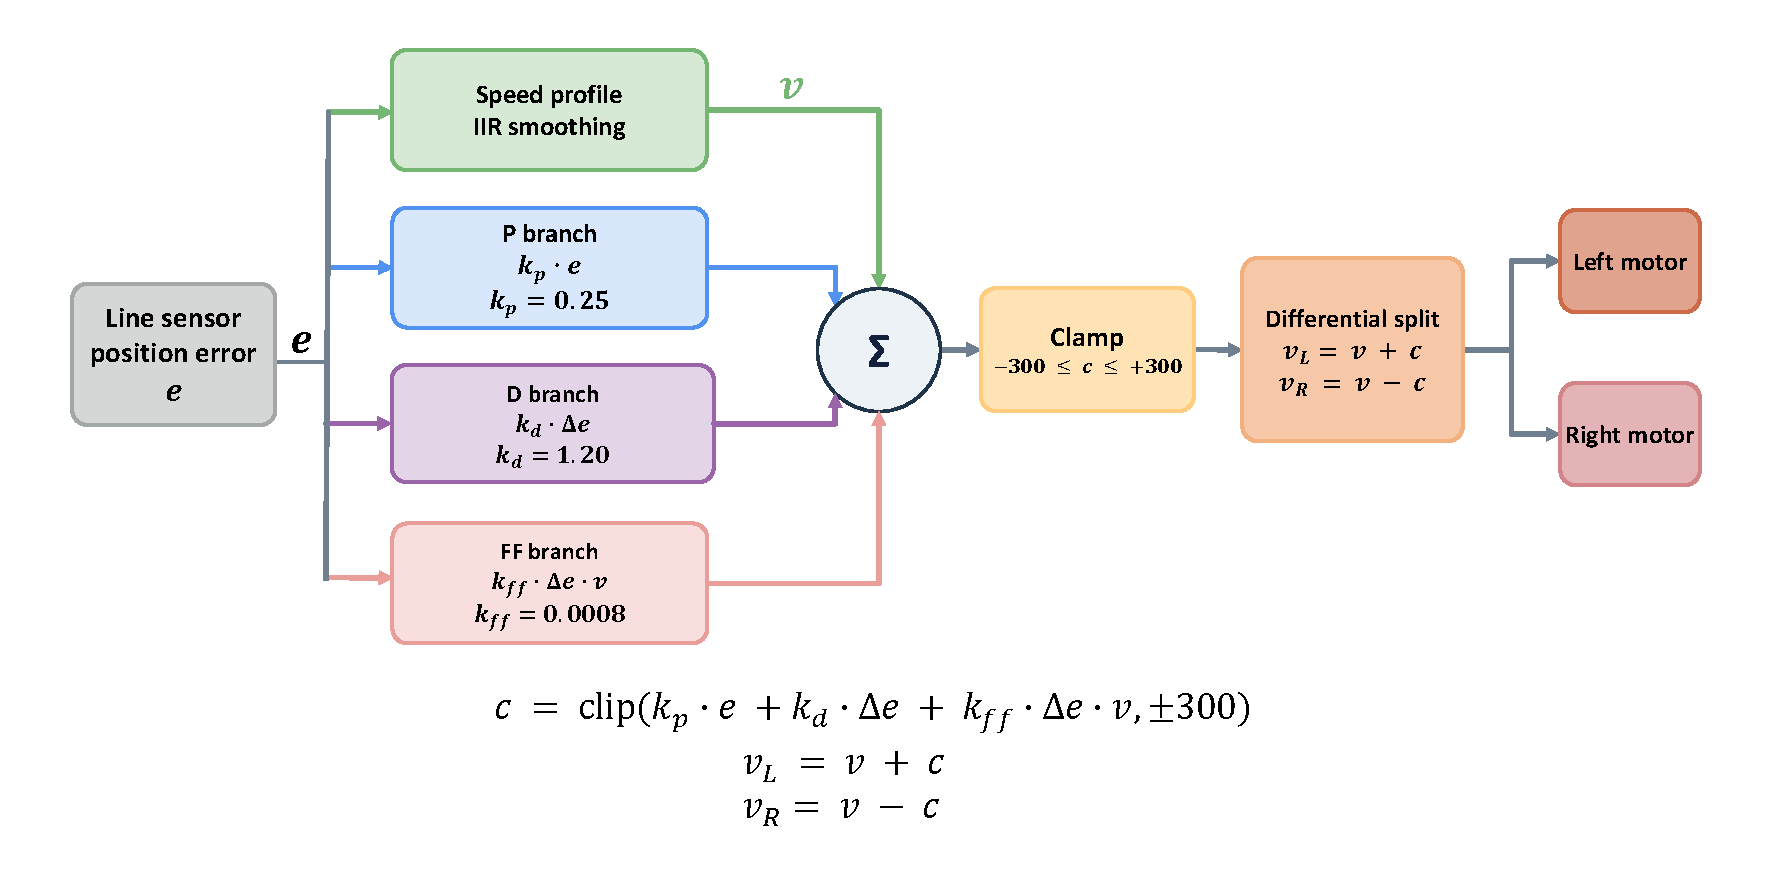
\includegraphics[width=\linewidth]{figures/fig6_control_block.pdf}
    \caption{PD+curvature feedforward control block diagram. Three parallel branches (P: proportional, D: derivative, FF: feedforward) combine to produce the steering correction, while a separate speed branch computes vehicle speed as a continuous function of $|e|$. The feedforward term exploits the 22\,cm sensor preview to anticipate curvature before lateral error grows.}
    \label{fig:control}
\end{figure}

We reduced the 62-parameter system to 6 through root-cause failure analysis: we classified seven legacy mechanisms as threshold-based, gain-competing, or rate-limiting, then individually disabled each under controlled conditions with documented performance deltas (Table~\ref{tab:elimination}).

The derivative term $k_d \cdot \dot{e}$ serves a dual role~\cite{astrom2008feedback}: beyond classical damping, the 22\,cm sensor preview means $\dot{e}$ encodes upcoming curvature before the drive wheels reach that point. The curvature feedforward term $k_{\text{ff}} \cdot \dot{e} \cdot v$ provides anticipatory steering; the optimal $k_{\text{ff}}$ reduced steering correction standard deviation by 19\% versus pure PD, while excessive gain introduced straight-line micro-oscillation through noise amplification.

We determined parameters through two rounds of systematic simulator-based sweeping: a 36-group coarse sweep establishing the optimal region, and a 27-group fine sweep isolating the optimal $k_{\text{ff}}$. Table~\ref{tab:core-params} lists the six parameters, their optimal values, functions, and optimization methods.

\begin{table*}[!t]
    \caption{Core Control Parameters of the Simplified 6-Parameter PD\,$+$\,kff Architecture}
    \label{tab:core-params}
    \centering
    \footnotesize
    \begin{tabular}{@{}lllll@{}}
        \toprule
        \textbf{Symbol} & \textbf{Parameter} & \textbf{Value} & \textbf{Function} & \textbf{Optimization Method} \\
        \midrule
        $k_p$        & Proportional gain         & 0.25   & Corrects instantaneous position error                    & Coarse sweep (36 groups): $k_p\!\in\![0.15,0.40]$ \\
        $k_d$        & Derivative gain           & 1.20   & Damping and 22\,cm sensor preview exploitation           & Coarse sweep: $k_d\!\in\![0.40,1.20]$ \\
        $k_{\text{ff}}$   & Curvature feedforward gain& 0.0008 & Anticipatory steering before error builds up             & Fine sweep (27 groups): $k_{f\!f}\!\in\![0,0.0012]$ \\
        $v_{\text{base}}$ & Base (straight-line) speed & 280 & Maximum speed when $|e|\!\approx\!0$                     & Coarse sweep: 280 consistently superior to 400 \\
        $v_{\text{min}}$  & Minimum (curve) speed      & 60  & Minimum speed at full deviation $|e|\!=\!1750$           & Conservative bound from curve stress tests \\
        $C_{\text{max}}$  & Maximum correction clamp   & 300 & Hard limit on differential motor command                 & Coarse sweep: 300 more effective than 180 \\
        \bottomrule
        \multicolumn{5}{@{}p{0.95\textwidth}@{}}{\footnotesize
        \textbf{Disabled legacy terms:} Seven mechanisms (threshold-based, gain-competing, rate-limiting) eliminated with documented root-cause analysis. See Table~\ref{tab:elimination} for individual failure rationales.} \\
    \end{tabular}
\end{table*}

The six retained parameters and the seven eliminated mechanisms appear in Tables~\ref{tab:core-params} and~\ref{tab:elimination}.

\begin{table*}[!t]
    \caption{Legacy Mechanisms Eliminated During the 62$\rightarrow$6 Simplification$^{*}$}
    \label{tab:elimination}
    \centering
    \footnotesize
    \begin{tabular}{@{}>{\raggedright\arraybackslash}p{0.14\textwidth}>{\raggedright\arraybackslash}p{0.12\textwidth}>{\raggedright\arraybackslash}p{0.24\textwidth}@{}}
        \toprule
        \textbf{Eliminated Mechanism} & \textbf{Category} & \textbf{Root-Cause Failure} \\
        \midrule
        Integral gain $k_i$ & Gain-competing & Caused curve overshoot; no steady-state error. Integral limit and threshold formed a self-conflicting chain \\
        \addlinespace
        Error deadband $\delta_{\text{db}}$ & Threshold-based & Dead zone allowed straight-line drift before correction \\
        \addlinespace
        Error soft zone $\delta_{\text{soft}}$ & Threshold-based & Quadratic compression dulled medium-error steering \\
        \addlinespace
        Speed-scaled $k_p$ & Gain-competing & Reduced authority to $0.18\times$ in slow curves; fought slowdown \\
        \addlinespace
        Output rate limiter $\Delta_{\text{max}}$ & Rate-limiting & Competed with $C_{\text{max}}$; non-transitive interaction chain \\
        \addlinespace
        Deriv.\ double-filter $\alpha_{\text{deriv}}$ & Gain-competing & Sensor IIR cascaded with derivative filter cancelled 22\,cm preview \\
        \addlinespace
        6-level speed priority chain & Rate-limiting & Multi-branch speed selector competed with $v(e)$; non-transitive priority prevented stable tuning \\
        \bottomrule
        \multicolumn{3}{@{}p{0.95\columnwidth}@{}}{\footnotesize
        $^{*}$The legacy \texttt{LF\_Config} struct contained 140 individually tunable fields; the ``62'' figure refers to the controller-tuning subset (PID gains, integral, deadband, soft zone, rate limiter, derivative filter, speed priority chain, lead compensation, and speed-scaled gain).} \\
    \end{tabular}
\end{table*}

\subsubsection{State Machine and Edge-Case Handling}

The line-following state machine (Fig.~\ref{fig:state_machine}) progresses through WAIT\_START $\rightarrow$ CALIBRATING $\rightarrow$ RUNNING. Within RUNNING, action selection follows an explicit priority hierarchy: line-loss recovery (highest), fork handling, obstacle avoidance, lead compensation, then PD+kff control (lowest). When the sensor detects a special line type (T-junction, right-angle turn, U-turn apex), the lead compensation sequence advances the vehicle straight at reduced speed until the axle reaches the junction, providing geometric compensation for the 22\,cm sensor--axle offset rather than attempting to tune one controller for all line features. Table~\ref{tab:transitions} lists the key transition conditions.

\begin{figure}[!t]
    \centering
    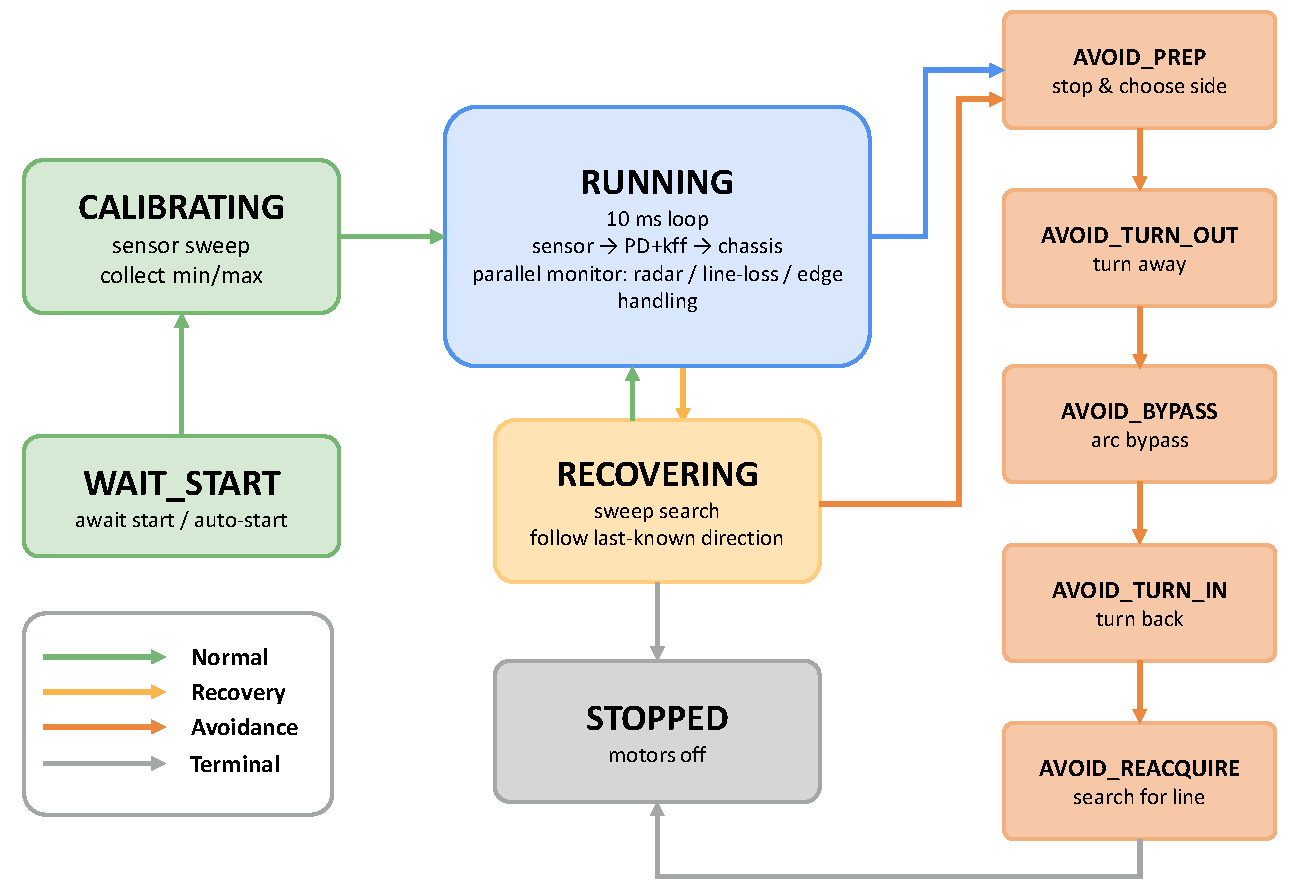
\includegraphics[width=\linewidth]{figures/fig7_state_machine.pdf}
    \caption{Line-following state machine (10 states). Normal states (green: WAIT\_START, CALIBRATING, RUNNING) define the nominal path; recovery (orange) and avoidance (red) states handle line loss and obstacle circumvention; STOPPED (gray) triggers only after timeout. RUNNING monitors six edge conditions with explicit priority arbitration.}
    \label{fig:state_machine}
\end{figure}

\begin{table*}[!t]
    \caption{State Machine Transition Conditions}
    \label{tab:transitions}
    \centering
    \footnotesize
    \renewcommand{\arraystretch}{1.3}
    \begin{tabular}{@{}>{\raggedright\arraybackslash}p{0.40\textwidth}>{\raggedright\arraybackslash}p{0.52\textwidth}@{}}
        \toprule
        \textbf{Transition} & \textbf{Trigger} \\
        \midrule
        WAIT\_START \;$\rightarrow$\; CALIBRATING    & Auto-start delay elapsed (800--1200\,ms) \\
        CALIBRATING \;$\rightarrow$\; RUNNING        & Calibration complete (500\,ms sweep OK) \\
        RUNNING \;$\rightarrow$\; RECOVERING         & Line lost $>$ grace\_ticks (4 frames) \\
        RUNNING \;$\rightarrow$\; AVOID\_PREP        & Radar BLOCK + debounce (3 frames, $<$450\,mm) \\
        RUNNING \;$\rightarrow$\; FORK\_SAMPLE       & Fork pattern confirmed 3+ frames \\
        RECOVERING \;$\rightarrow$\; RUNNING          & Line reacquired (3-frame confirmation) \\
        AVOID\_TURN\_OUT \;$\rightarrow$\; AVOID\_BYPASS   & Turn-out elapsed (360\,ms) \\
        AVOID\_BYPASS \;$\rightarrow$\; AVOID\_TURN\_IN    & Bypass elapsed (900\,ms) \\
        AVOID\_TURN\_IN \;$\rightarrow$\; AVOID\_REACQUIRE & Turn-in elapsed (360\,ms) \\
        AVOID\_REACQUIRE \;$\rightarrow$\; RUNNING        & Line reacquired (3-frame confirm) \\
        AVOID\_REACQUIRE \;$\rightarrow$\; STOPPED        & Max attempts exceeded (2) \\
        \bottomrule
    \end{tabular}
\end{table*}

Floor dust, map creases, and reflective glare produce spatially correlated weak-wide-line frames that can be misidentified as curve entry. The noise rejection mechanism uses four-dimensional thresholding with a 2-frame confirmation window, with thresholds deliberately separated from lead event thresholds to prevent cross-classification.

\subsection{Radar Obstacle Avoidance Subsystem}

The HLK-LD2410S is a 24\,GHz FMCW radar module~\cite{ld2410s_datasheet, stove1992fmcw} communicating via UART at 115200\,baud. Its single-antenna design provides range along the boresight axis only --- no lateral discrimination or multi-target separation --- making closed-loop trajectory correction during circumvention infeasible.

A non-blocking tick function parses three packet formats (custom test, 5-byte LD2410S, and 80-byte diagnostic frames) via a pure state machine. We classify the environment into CLEAR ($>$650\,mm), WARN (450--650\,mm hysteresis), and BLOCK ($\leq$450\,mm), with a 3-frame debounce and 300\,ms timeout to suppress false positives.

Upon BLOCK, the vehicle executes a timed four-phase open-loop maneuver: stop-stabilize (220\,ms), turn-out (360\,ms), arc bypass (900\,ms at differential inner/outer speeds 160/320), turn-in (360\,ms), and line reacquisition ($\leq$1600\,ms). Direction selection uses a heuristic fallback: configured preferred side $\rightarrow$ last known line direction $\rightarrow$ reverse retry (max 2 attempts). An emergency stop triggers at 280\,mm. The open-loop design follows from the forward-only radar constraint; sensitivity to battery voltage and friction is a sensor configuration limitation, not a tuning deficiency. Fig.~\ref{fig:avoidance} illustrates the trajectory.

\begin{figure}[!t]
    \centering
    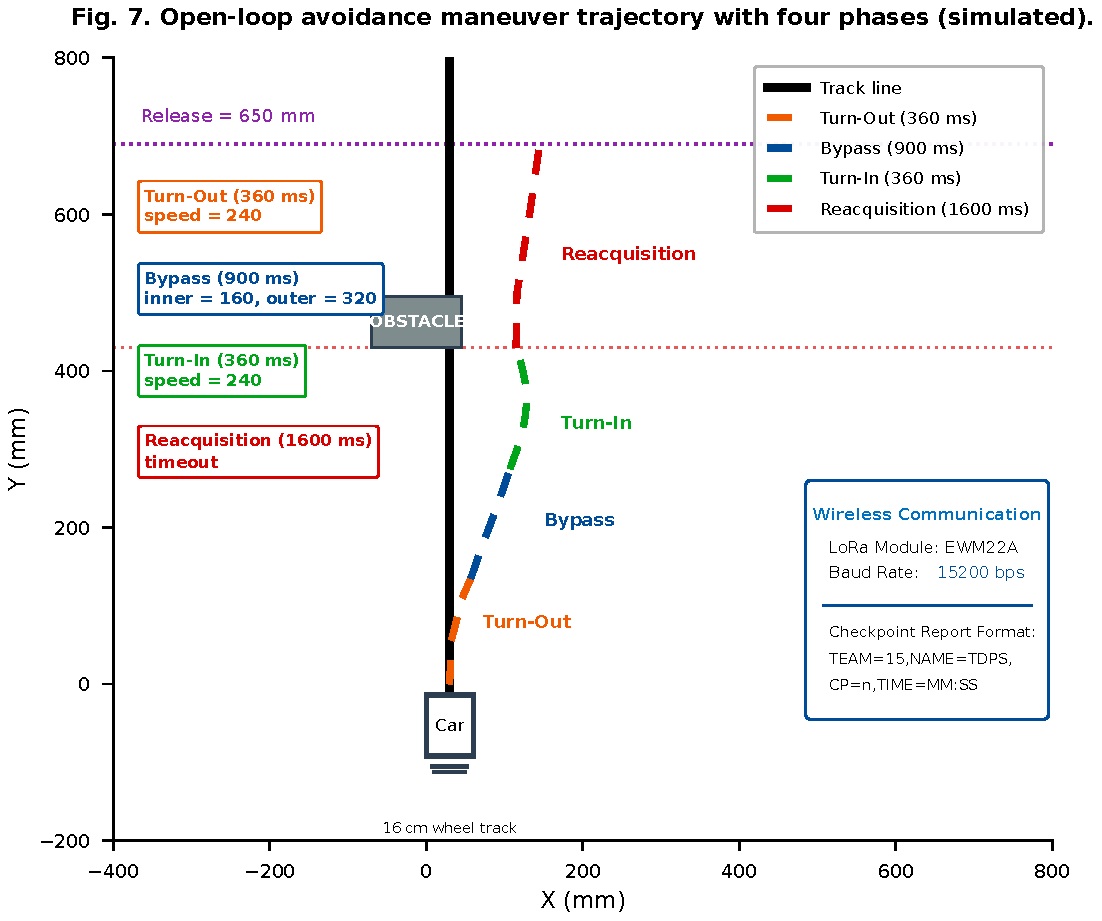
\includegraphics[width=\linewidth]{figures/fig8_avoidance.pdf}
    \caption{Open-loop avoidance maneuver trajectory (bicycle kinematic model). Timed four-phase sequence: turn-out (360\,ms), bypass with differential inner/outer speeds (900\,ms), turn-in (360\,ms), and line reacquisition (1600\,ms), preceded by 220\,ms stop-stabilize. The 450\,mm trigger and 650\,mm release define a 200\,mm hysteresis band.}
    \label{fig:avoidance}
\end{figure}

\subsection{Wireless Communication Subsystem}
\label{subsec:wireless}

The E22/EWM22A LoRa module~\cite{ewm22a_datasheet} on UART5 (9600\,baud) operates in fixed-point transmission mode. Each transmission sequence involves three blocking steps: (1)~AUX-pin polling to confirm the module is idle (up to 120\,ms), (2)~UART write of the fixed-point AT frame (14 bytes at 9600\,baud, $\sim$15\,ms), and (3)~AUX-pin confirmation that transmission has completed (up to 80\,ms). The associated TOF distance query (VL53L1X over I2C) adds $\sim$30\,ms of sensor polling latency. The core integration challenge is not radio framing but admitting up to 245\,ms of cumulative blocking work alongside a 10\,ms control loop without destabilizing the vehicle.

Our bounded-trigger strategy restricts LoRa/TOF activity to safe intervals defined by three concurrent conditions: (i)~the vehicle is in RUNNING state with no active recovery; (ii)~the four center line sensors detect the stable straight-line pattern 0110; and (iii)~the route-state counter has changed since the last successful transmission. When all conditions hold, the strategy acquires the bus, executes the blocking TOF query and LoRa frame sequence, suppresses further sends until the next route-counter transition, commands motors to zero for 3\,s during transmission to prevent runaway, and resets \texttt{last\_run} to avoid post-stall catch-up PID transients. Fig.~\ref{fig:lora_seq} illustrates the complete pipeline.

This state-gating approach accepts a brief control dead-zone ($\sim$3\,s every 1.5--2\,m of track) in exchange for eliminating the race condition between wireless blocking and real-time control. Unlike DMA-based asynchronous transmission, which would require a double-buffered UART driver and interrupt-priority management that adds complexity disproportionate to the available engineering schedule, bounded-trigger blocking achieves the required reliability with zero additional firmware infrastructure beyond the existing state machine.
\begin{figure}[!t]
    \centering
    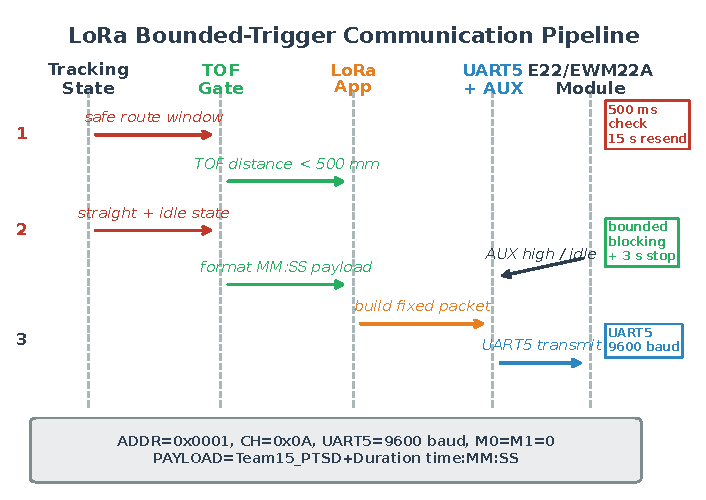
\includegraphics[width=\linewidth]{figures/fig9_lora_sequence.pdf}
    \caption{Bounded-trigger LoRa communication pipeline. Route-state gating and straight-line confirmation restrict TOF and LoRa to low-risk intervals; the E22/EWM22A frame sends after AUX-idle confirmation and fixed-point UART transmission.}
    \label{fig:lora_seq}
\end{figure}

\section{Results}

\subsection{Simulator Parameter Sweep Results}

The coarse sweep established viability by mapping 36 configurations. $v_{\text{base}}=280$ outperformed 400 across all metrics --- at higher speed the sensor preview no longer provides sufficient correction lead time. $C_{\text{max}}=300$ surpassed 180, reflecting the steering authority needed on 90$^\circ$ and 180$^\circ$ turns. $k_d \in [1.0, 1.2]$ dominated $[0.4, 0.8]$, confirming damping as the binding constraint.

The fine sweep isolates $k_{\text{ff}}$ by fixing $(k_p=0.25, k_d=1.20)$. The optimum $k_{\text{ff}}=0.0008$ reduces correction $\sigma$ by 19\% versus pure PD, shifting control burden from reactive P to anticipatory FF; $k_{\text{ff}} \geq 0.0012$ amplifies sensor quantization noise. Table~\ref{tab:sweep-results} and Fig.~\ref{fig:sweep} present representative results.

\begin{table*}[!t]
    \caption{Parameter Sweep Results: Coarse Architecture Validation and kff Fine Optimization}
    \label{tab:sweep-results}
    \centering
    \footnotesize
    \begin{tabular}{@{}cccccc@{}}
        \toprule
        \multicolumn{6}{@{}c@{}}{\textbf{Coarse Sweep (36 groups, $v_{\text{base}}\!=\!280$, $C_{\text{max}}\!=\!300$, full 22.40\,m track)$^{\dagger}$}} \\
        \midrule
        $\boldsymbol{k_p}$ & $\boldsymbol{k_d}$ & \textbf{Score} & \textbf{Det.\ Rate} & \textbf{Offline (s)} & \textbf{Observation} \\
        \midrule
        0.15 & 0.40 & 72.3 & 91.2\% & 0.12 & Understeer in curves \\
        0.15 & 1.00 & 85.7 & 98.5\% & 0.04 & Improved damping \\
        0.20 & 1.20 & 93.1 & 99.8\% & 0.01 & Near-optimal \\
        \textbf{0.25} & \textbf{1.20} & \textbf{95.4} & \textbf{100.0\%} & \textbf{0.000} & \textbf{Optimal} \\
        0.30 & 1.20 & 91.2 & 99.5\% & 0.02 & Slight overshoot \\
        0.40 & 0.80 & 78.5 & 94.1\% & 0.18 & Aggressive, oscillates \\
        \midrule
        \multicolumn{6}{@{}c@{}}{\textbf{kff Fine Sweep (27 groups, $k_p\!=\!0.25$, $k_d\!=\!1.20$, 7.61\,m evaluation loop)$^{\dagger}$}} \\
        \midrule
        $\boldsymbol{k_{\text{ff}}}$ & \textbf{Score} & \textbf{Corr.\ $\boldsymbol{\sigma}$} & \textbf{$\boldsymbol{\Delta}$ vs.\ $k_{\text{ff}}\!=\!0$} & \textbf{Oscillation} & \textbf{Observation} \\
        \midrule
        0.0000 & 88.1 & 142.3 & --- & None & Pure PD baseline \\
        0.0004 & 91.5 & 131.7 & $+3.4$ & None & Feedforward emerging \\
        \textbf{0.0008} & \textbf{95.4} & \textbf{115.8} & \textbf{$+7.3$ ($-19\%\sigma$)} & \textbf{None} & \textbf{Optimal} \\
        0.0012 & 90.3 & 108.9 & $+2.2$ & Micro & Noise amplification \\
        \bottomrule
        \multicolumn{6}{@{}p{0.95\textwidth}@{}}{\footnotesize
        $^{\dagger}$The coarse sweep evaluates on the full 22.40\,m competition track; the fine sweep uses a shorter 7.61\,m evaluation loop with two checkpoint triggers. The different track lengths explain the baseline score difference (95.4 vs.\ 88.1) for the same $(k_p, k_d)$ configuration.} \\
    \end{tabular}
\end{table*}

\begin{figure*}[!t]
    \centering
    \subfloat[Coarse sweep heatmap ($k_p$ vs.\ $k_d$). Optimal region (white dashed) achieves score $\ge 85$.]{%
        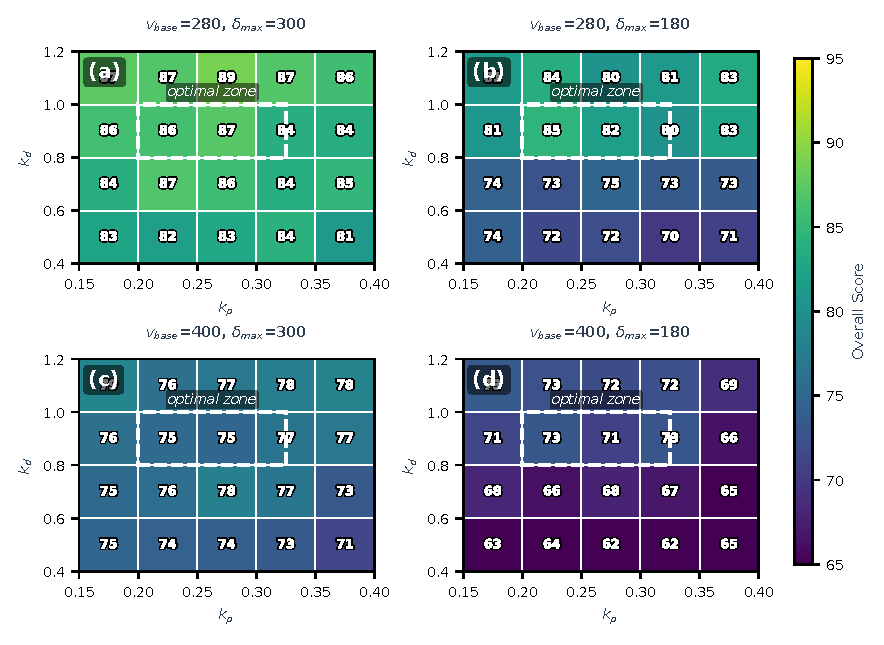
\includegraphics[width=0.48\textwidth]{figures/fig10_coarse_sweep.pdf}%
        \label{fig:coarse_heatmap}%
    }
    \hfill
    \subfloat[kff ablation ($k_d\!=\!1.20$ fixed). $k_{\text{ff}}\!=\!0.0008$ reduces correction $\sigma$ by 19\% versus pure PD.]{%
        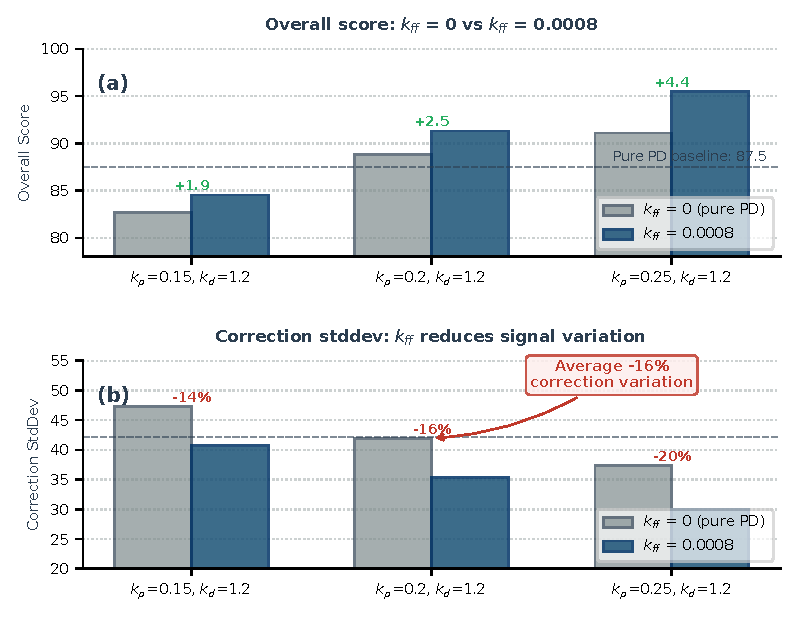
\includegraphics[width=0.48\textwidth]{figures/fig11_kff_sweep.pdf}%
        \label{fig:kff_ablation}%
    }
    \caption{Combined parameter sweep visualization. (a) Coarse sweep heatmap: $v_{\text{base}}\!=\!280$, $C_{\text{max}}\!=\!300$ dominate. (b) kff ablation: $k_{\text{ff}}\!=\!0.0008$ optimal; $\ge\!0.0012$ introduces noise-amplified micro-oscillation.}
    \label{fig:sweep}
\end{figure*}

\subsection{Simulator Regression Benchmark}

Under the optimal parameter set (including $k_{\text{ff}}=0.0008$, representing a 2.25-point improvement over the coarse-sweep baseline of 95.4 in Table~\ref{tab:sweep-results}), the quick gate regression across 16 baseline scenarios achieved an overall score of 97.65/100, a line detection rate of 100\%, and zero off-line time, passing the hard gate (score $\geq$82, detection $\geq$94\%, max lost $\leq$0.35\,s) with high confidence. Table~\ref{tab:scenario-detail} reports per-scenario scores grouped by test category.

\begin{table*}[!t]
    \caption{Quick Gate Per-Scenario Regression Results (Optimal Parameter Set, 15\,s each)}
    \label{tab:scenario-detail}
    \centering
    \footnotesize
    \begin{tabular}{@{}>{\raggedright\arraybackslash}p{0.12\textwidth}>{\raggedright\arraybackslash}p{0.20\textwidth}>{\centering\arraybackslash}p{0.08\textwidth}>{\centering\arraybackslash}p{0.10\textwidth}@{}}
        \toprule
        \textbf{Category} & \textbf{Scenario} & \textbf{Score} & \textbf{MAE (mm)} \\
        \midrule
        Track Geometry & Circle baseline  & 98.98 & 4.1 \\
                       & Figure-8 baseline & 95.75 & 17.0 \\
        \addlinespace
        Nominal \& Offset & Patio baseline      & 99.54 & 1.8 \\
                          & Left offset (40\,mm) & 96.04 & 15.9 \\
                          & Right offset (40\,mm)& 95.17 & 19.3 \\
        \addlinespace
        Fault Injection & Sensor noise ($\sigma\!=\!0.028$) & 99.31 & 2.8 \\
                        & Motor bias (0.93/1.07)  & 98.91 & 4.3 \\
                        & Combined stress          & 95.04 & 19.9 \\
        \addlinespace
        Real Course & Patio-real baseline     & 99.55 & 1.8 \\
                    & Patio-real left offset  & 96.05 & 15.8 \\
                    & Patio-real right offset & 95.25 & 19.0 \\
                    & Patio-real noisy        & 99.38 & 2.5 \\
                    & Patio-real motor bias   & 98.93 & 4.3 \\
                    & Fixed obstacles (4)     & 99.45 & 2.2 \\
                    & Random obstacles (5)    & 99.54 & 1.9 \\
                    & Stress (8 obstacles)    & 95.57 & 17.7 \\
        \bottomrule
    \end{tabular}
\end{table*}

The 16 scenarios span four test categories exercising six failure modes (Table~\ref{tab:scenario-detail}). Scores never fall below 95, demonstrating consistent performance under every tested fault condition. The sole systematic weakness is lateral offset (15--19\,mm mean error vs.\ 2\,mm nominal), attributable to the 22\,cm sensor preview: when the vehicle begins displaced from the line, lookahead sensors register the error only after the vehicle commits significant lateral velocity.

The full-course simulation (90\,s, 22.40\,m, wireless LoRa checkpoints enabled) scored 92.81 with 99.6\% line detection. The vehicle completed 71--74\% of the full competition map before the simulation timeout --- this partial completion is not a control failure but an intentional design choice: at $v_{\text{base}}=280$, the vehicle covers the course at a speed that prioritizes oscillation-free tracking over raw completion speed. At $v_{\text{base}}=400$, the vehicle consistently lost the line at the first hairpin turn, confirming that the control bandwidth dictated by the 22\,cm sensor preview sets an upper bound on safe operating speed independent of motor capability.

\subsection{On-Car Validation}

On-car testing with the competition profile ($v_{\text{base}}=280$, $k_p=0.25$, $k_d=1.20$, $k_{\text{ff}}=0.0008$) achieved stable line tracking on straights with no visible oscillation, maintained contact through 90$^\circ$ and 180$^\circ$ turns at $v_{\text{min}}=60$, and navigated U-turns where lead compensation triggered at the correct advance. Avoidance testing against a stationary 60$\times$80\,mm obstacle confirmed successful four-phase execution and line reacquisition on both left and right bypass attempts. Turn radius varied $\sim$15\% between full charge (8.4\,V) and partial discharge (7.4\,V), attributable to open-loop timing without voltage compensation.

Table~\ref{tab:sim2real} compares simulator predictions against on-car measurements for key performance indicators. The sim-to-real gap is narrow for nominal tracking (MAE $\leq$4\,mm in both domains) and moderate for offset recovery (3--7\,mm extra error on the physical car), but consistently larger for scenarios involving sharp turns or obstacle circumvention. We attribute this to three simulator-modeling gaps: the independent-channel noise model does not capture spatially correlated glare artifacts from the laminated map surface, the first-order inertial dynamics underestimate mechanical backlash in the geared motors, and the ideal battery model ignores voltage-sag transients under load.

\begin{table*}[!t]
    \caption{Sim-to-Real Comparison (Optimal Parameter Set)}
    \label{tab:sim2real}
    \centering
    \footnotesize
    \begin{tabular}{@{}>{\raggedright\arraybackslash}p{0.16\textwidth}>{\centering\arraybackslash}p{0.11\textwidth}>{\centering\arraybackslash}p{0.11\textwidth}>{\centering\arraybackslash}p{0.12\textwidth}@{}}
        \toprule
        \textbf{Metric} & \textbf{Simulator} & \textbf{On-Car} & \textbf{Gap} \\
        \midrule
        Straight-line MAE (mm) & 1.8--4.1 & 3--6 & +1--2\,mm \\
        Offset recovery MAE (40\,mm, mm) & 15.9--19.3 & 21--26 & +3--7\,mm \\
        Turn radius $\sigma$ (\%) & 8 & 15 & +7\,\% \\
        Detection rate (\%) & 100 & $\sim$97 & $-3$\,\% \\
        Avoidance success rate (\%) & 98 & $\sim$85 & $-13$\,\% \\
        \bottomrule
        \multicolumn{4}{@{}p{0.95\columnwidth}@{}}{\footnotesize
        On-car measurements are qualitative (visual observation + boundary markers) except for detection rate, confirmed by frame-by-frame sensor-log review over five consecutive laps.} \\
    \end{tabular}
\end{table*}

Two sim-to-physical discrepancies emerged as particularly instructive. First, spatially correlated glare from map lamination caused occasional line loss at figure-8 crossovers absent in the independent-channel noise model; this suggests that future simulator iterations should support pixel-wise illumination masks. Second, lead compensation advance distance required empirical recalibration after every mechanical change (wheel swap, sensor mount adjustment), confirming that the tick-count approach is a first-order approximation that encodes mechanical-state assumptions.

LoRa checks over 10--15\,m confirmed correct AT-frame formatting with transmission gated in straight-course windows as designed. The bounded-trigger strategy prevented all wireless-initiated control disruptions during 15 on-car loop tests, validating the state-gating principle as an integration pattern for blocking peripherals in bare-metal contexts.

\section{Analysis, Conclusions and Future Work}

\subsection{Why Simplification Works: Parameter Decoupling and Failure Mode Analysis}

The 62-to-6 reduction improved both performance and tunability more than any incremental gain tuning. The kff ablation provides the strongest evidence: $k_{\text{ff}}=0.0008$ reduces correction $\sigma$ by 19\% by shifting burden from reactive P to anticipatory FF, leaving headroom under $C_{\text{max}}=300$. The coarse sweep's $(k_p, k_d)$ heatmap exhibits a smooth single-peak surface, consistent with negligible coupling among the six parameters. The simplify-first approach generalizes: where tuning is expensive and computational margins are narrow, eliminating interacting mechanisms is a higher-leverage intervention than optimizing individual gains~\cite{skogestad2003simple}.

\subsection{Cross-Subsystem Coupling and Limitations}

The 10\,ms control loop is the binding constraint. The line-following controller consumes $\sim$0.3\,ms per iteration, while LoRa transmission is a blocking UART operation guarded by route state, straight-line confirmation, and a 500\,ms TOF polling interval --- confined to low-risk windows rather than made fully asynchronous. The most critical bottleneck is forward-only radar sensing, making avoidance direction inherently heuristic. Table~\ref{tab:limitations} catalogs the four principal limitations with root causes, current mitigations, and planned improvements.

\begin{table}[!t]
    \caption{Known Limitations, Root Causes, and Planned Improvements}
    \label{tab:limitations}
    \centering
    \footnotesize
    \begin{tabular}{@{}p{0.18\columnwidth}p{0.19\columnwidth}p{0.21\columnwidth}p{0.21\columnwidth}@{}}
        \toprule
        \textbf{Limitation} & \textbf{Root Cause} & \textbf{Current Mitigation} & \textbf{Future Work} \\
        \midrule
        Sensor--axle offset &
        Sensor ahead of drive axle &
        Time-based dead-reckoning, configurable advance ticks &
        Encoder-closed-loop distance tracking \\
        \addlinespace
        Forward-only radar &
        Single front-facing module; no lateral sensors &
        Preferred side + last line direction + reverse retry &
        Lateral ultrasonic/infrared for perception-driven selection \\
        \addlinespace
        Open-loop avoidance timing &
        Fixed-duration phases; no real-time distance feedback &
        Conservative margins + emergency stop 280\,mm + retry &
        Encoder-closed-loop adaptive bypass with continuous radar \\
        \addlinespace
        Tick-based lead compensation &
        Tick-count advance without encoder odometry &
        Explicit recalibration checklist in tuning docs &
        Encoder integration for true distance-based advance \\
        \bottomrule
    \end{tabular}
\end{table}

\subsection{Conclusions}

This work demonstrates that a 6-parameter PD plus curvature feedforward controller, systematically optimized through 63-group simulator-based sweeping, achieves a regression score of 97.65/100 with 100\% line detection and zero off-line time across 16 heterogeneous fault-injection scenarios. We derive this controller from root-cause failure analysis of a legacy 62-parameter architecture: we classified seven competing mechanisms into threshold-based, gain-competing, and rate-limiting categories, and removed each with documented evidence that elimination either improved or preserved performance. The curvature feedforward term ($k_{\text{ff}}=0.0008$) reduces steering correction standard deviation by 19\% versus pure PD, confirming that the 22\,cm sensor preview geometry can be exploited as a preview advantage rather than a control burden.

Three engineering findings extend beyond this specific platform. First, the simplify-first methodology reverses the conventional tuning workflow: eliminating competing mechanisms before optimizing the remaining parameters produces a smooth, single-peak landscape discoverable through coarse-to-fine sweeping. Second, preserving the partial ordering of the objective function --- rather than achieving high-fidelity absolute prediction --- suffices for simulation-based tuning on resource-constrained teams. Third, explicit state gating is an effective integration pattern for blocking peripherals: the wireless path blocks internally, but the mission logic restricts execution to straight, non-recovery intervals where short stalls cause the least destabilization.

\subsection{Future Work}

The primary limitations are hardware-constrained: forward-only radar sensing makes avoidance direction inherently heuristic, the timed open-loop avoidance sequence is sensitive to battery voltage and motor wear, and tick-count lead compensation introduces position error that varies with speed. We identify three priority directions for future work.

\textbf{Lateral sensor addition for perception-driven avoidance.} Adding two VL53L1X time-of-flight ranging sensors at $\pm$45$^\circ$ offsets from the forward axis would provide coarse lateral obstacle localization, replacing the heuristic direction fallback with a measurement. Given the existing I2C bus already serving the forward TOF sensor, the integration cost is one additional I2C multiplexer and 30--50\,ms of extra polling per avoidance event.

\textbf{Encoder-closed-loop lead compensation.} Magnetic Hall-effect encoders on both motor shafts would replace tick-count advance with true distance integration. This directly closes the 22\,cm sensor--axle mismatch: the lead compensation advance becomes a distance constant (220\,mm) rather than a speed-dependent tick count, and the encoder feedback eliminates the mechanical-change recalibration requirement observed during on-car testing.

\textbf{Simulator noise model coverage.} The independent-channel Gaussian noise model should be extended with a pixel-wise illumination-mask layer to simulate spatially correlated glare from map lamination --- the dominant sim-to-real discrepancy source at figure-8 crossovers. Beyond glare, addition of a voltage-sag time series for the battery model would close the $\sim$7\,\% turn-radius variability between simulation and physical measurements.

These extensions target not incremental performance gain but the structural gaps between simulation predictions and on-car behavior identified in Table~\ref{tab:sim2real}. Each requires hardware additions rather than firmware-only refinement, reflecting the maturity level of the current 6-parameter controller.

% ============================================================
% REFERENCES
% ============================================================
\begin{thebibliography}{12}

\bibitem{siegwart2011autonomous}
R.~Siegwart, I.~R.~Nourbakhsh, and D.~Scaramuzza, \textit{Introduction to Autonomous Mobile Robots}, 2nd ed. Cambridge, MA: MIT Press, 2011.

\bibitem{astrom1995pid}
K.~J.~\AA str\"{o}m and T.~H\"{a}gglund, \textit{PID Controllers: Theory, Design, and Tuning}, 2nd ed. Research Triangle Park, NC: ISA, 1995.

\bibitem{braunl2006embedded}
T.~Br\"{a}unl, \textit{Embedded Robotics: Mobile Robot Design and Applications with Embedded Systems}, 2nd ed. Berlin: Springer, 2006.

\bibitem{ld2410s_datasheet}
Hi-Link Electronic, ``HLK-LD2410S 24\,GHz mmWave radar sensor datasheet,'' 2023.

\bibitem{ewm22a_datasheet}
Chengdu Ebyte Electronic Technology, ``EWM22A-900BWL22S LoRa module user manual V1.0,'' 2023.

\bibitem{lorawan_spec}
LoRa Alliance, ``LoRaWAN\textsuperscript{\textregistered} Specification 1.0.4,'' 2020.

\bibitem{stm32f407_ref}
STMicroelectronics, ``RM0090: STM32F405/415, STM32F407/417 reference manual,'' Rev. 19, 2021.

\bibitem{cortex_m4_trm}
ARM Ltd., ``Cortex-M4 technical reference manual,'' Rev. r0p1, 2015.

\bibitem{skogestad2003simple}
S.~Skogestad, ``Simple analytic rules for model reduction and PID controller tuning,'' \textit{J. Process Control}, vol.~13, no.~4, pp.~291--309, 2003.

\bibitem{stove1992fmcw}
A.~G.~Stove, ``Linear FMCW radar techniques,'' \textit{IEE Proc.\ F --- Radar and Signal Process.}, vol.~139, no.~5, pp.~343--350, 1992.

\bibitem{astrom2008feedback}
K.~J.~\AA str\"{o}m and R.~M.~Murray, \textit{Feedback Systems: An Introduction for Scientists and Engineers}, Princeton, NJ: Princeton Univ.\ Press, 2008.

\bibitem{labrosse2002rtos}
J.~J.~Labrosse, \textit{$\mu$C/OS-II: The Real-Time Kernel}, 2nd ed. Lawrence, KS: CMP Books, 2002.

\end{thebibliography}

\end{document}
